\documentclass[11pt]{article}

%% ====================================================================
%% The United States bloc of the Monetary-Financial-Fiscal Macromodel:
%% the estimated model and its international linkages, written down the
%% way the VAR literature does it.
%%
%% Accuracy contract: every equation and every number in this note was
%% extracted from the SHIPPED artifacts and source files of the deployed
%% tool (branch improve-live), never from memory:
%%   app/public/data/bvar/US/{spec,companion_mean}.json   (the live model)
%%   app/public/data/bvar/gvar/weights_full.json           (trade weights)
%%   app/public/data/bvar/gvar/coupling_default.json.gz    (rho, dim, M)
%%   pipeline/export_bvar_gvar24_loop.m                    (estimator)
%%   BVAR/MFBVAR/cgl_bvarV5.m, GLPreplicationWeb/bvarGLPmf.m, Support/BVAR.m
%%   app/src/lib/compute/{gvarSolve,kalman}.ts             (solve-time linkage)
%% File and line references are given in footnotes where the
%% correspondence matters. Reported coefficients are posterior means
%% recomputed from the shipped companion_mean.json.
%%
%% Build: lualatex MFFM_US_bloc_model.tex; bibtex; 2x lualatex.
%% ====================================================================

\usepackage[margin=2.5cm]{geometry}
\usepackage{amsmath,amsfonts,amssymb}
\usepackage{mathtools}
\usepackage{graphicx}
\usepackage{array}
\usepackage{booktabs,longtable}
\usepackage[round,authoryear]{natbib}
\usepackage{hyperref}
\hypersetup{
  pdfpagelayout=OneColumn, pdfstartview=Fit, pdfpagemode=UseNone,
  colorlinks=true, citecolor=blue, filecolor=blue,
  linkcolor=blue, urlcolor=blue}
\usepackage{enumitem}
\usepackage{setspace}
\onehalfspacing
\usepackage{float}
\usepackage{caption}
\usepackage{xcolor}
\usepackage{microtype}
\usepackage{tikz}
\usetikzlibrary{arrows.meta,positioning,fit,calc,decorations.pathreplacing}
\microtypesetup{expansion=false}

\newcommand{\code}[1]{\texttt{\small #1}}
\definecolor{blkblue}{RGB}{48,91,150}
\definecolor{blksoft}{RGB}{235,241,249}
\definecolor{blkgray}{RGB}{244,245,247}
\definecolor{blkred}{RGB}{150,45,45}

\title{The United States Bloc of the Monetary-Financial-Fiscal Macromodel:\\
The Estimated Model and Its International Linkages}
\author{M\'aty\'as Farkas\thanks{International Monetary Fund. This note documents the deployed
model exactly as shipped; every equation was checked against the implementation
(\code{pipeline/*.m}, \code{app/src/lib/compute/*.ts}) and every number recomputed from the
shipped data artifacts. It accompanies the full user manual (\emph{A guide to the
Monetary-Financial-Fiscal Macromodel}), whose notation it follows.}}
\date{July 16, 2026}

\begin{document}
\maketitle

\begin{abstract}
\noindent This note writes down, in the standard notation of the VAR literature, the model the
MFFM estimates for the United States and the exact channels through which foreign variables feed
into it. The US bloc is a 40-variable Bayesian VAR(3): 37 domestic series plus three
trade-weighted foreign aggregates (``stars'') --- foreign demand, foreign inflation, and a foreign
short rate --- that enter as \emph{endogenous} columns with their own equations, not as weakly
exogenous regressors. Foreign information reaches the domestic block through three explicit
channels: the $37\times3$ lag blocks on the stars, the innovation covariance between domestic and
star residuals, and --- at solve time --- the conditioning of the star paths on the other 32
coupled economies' solutions through a linear fixed point $x = Mx + d$ with spectral radius
$\rho(M)=0.947$. All coefficients reported here are posterior means read from the shipped model
files.
\end{abstract}

\section{The model in one paragraph}

The United States is one of 33 coupled blocs in the MFFM's global system. Its bloc is a
constant-coefficient VAR(3) in $n=40$ variables estimated on $T=110$ quarters (1998Q3--2025Q4)
under a hierarchical Minnesota prior \citep{Litterman1986,Giannone2015}, with the 2020Q2--Q4
macro observations treated as missing data and imputed by a Durbin--Koopman simulation smoother
inside the Gibbs sampler \citep{DurbinKoopman2002,TannerWong1987}. Three of the 40 variables are
constructed trade-weighted foreign aggregates whose historical values are rebuilt from the other
blocs' completed panels at every sweep of an outer EM-style iteration, and whose future paths are
\emph{pinned} to the other blocs' solutions whenever a coupled (global) solve is requested. This
note states each of those objects exactly.

\section{The US VAR}\label{sec:var}

\subsection{The system}

Let $y_t \in \mathbb{R}^{40}$ collect the US variables of Table~\ref{tab:roster} in the order
shipped. The estimated model is the closed reduced-form VAR($p$) with intercept,
\begin{equation}\label{eq:var}
  y_t \;=\; c \;+\; \sum_{\ell=1}^{p} B_\ell\, y_{t-\ell} \;+\; u_t,
  \qquad u_t \sim \text{i.i.d.}\ \mathcal{N}(0,\Sigma),
  \qquad p=3,
\end{equation}
with $c \in \mathbb{R}^{40}$, $B_\ell \in \mathbb{R}^{40\times40}$, and
$\Sigma \in \mathbb{R}^{40\times40}$ symmetric positive definite. The estimation sample is
$t = 1998\text{Q}3, \dots, 2025\text{Q}4$ ($T=110$ rows; the regression conditions on the first
$p=3$).\footnote{Sample and dimensions from the shipped
\code{app/public/data/bvar/US/spec.json} ($n=40$), \code{companion\_mean.json}
($\hat\beta$: $121\times40$, $\hat\Sigma$: $40\times40$, \code{lags}: 3) and
\code{coverage\_manifest.json} (estimation sample 1998Q3--2025Q4, 110 periods). The deployed
\emph{display} origin is one quarter later (2026Q1): the production data shift appended one
observed quarter and re-anchored the forecast origin without re-estimating the companion, so
forecasts shown in the tool run 2026Q2--2031Q1 ($H=20$).}

Variables tagged \emph{log} in Table~\ref{tab:roster} enter in the $100\ln$ space,
$\ell_t = 100\ln Y_t$, so that the app's displayed quarter-on-quarter annualized growth is
$g_t = 4\,(\ell_t - \ell_{t-1}) = 400\,\Delta \ln Y_t$; variables tagged \emph{level} (rates,
ratios to GDP, survey indices) enter untransformed. The three foreign stars are stored as
\emph{level} columns whose values are themselves already annualized-percent constructs
(Section~\ref{sec:stars}).

\subsection{The domestic/foreign partition}\label{sec:partition}

Partition $y_t$ into the $n_x = 37$ domestic variables and the $n_* = 3$ foreign stars,
\begin{equation}\label{eq:partition}
  y_t \;=\;
  \begin{pmatrix} x_t \\ x^{*}_t \end{pmatrix},
  \qquad
  x^{*}_t \;=\;
  \begin{pmatrix}
    \mathrm{ROWDEM}_t \\ \mathrm{ROWINF}_t \\ \mathrm{ROWFIN}_t
  \end{pmatrix}
  \;=\;
  \begin{pmatrix}
    \text{foreign demand} \\ \text{foreign inflation} \\ \text{foreign short rate}
  \end{pmatrix},
\end{equation}
where $x_t$ stacks the macro core (columns 0--19), the financial block (20--31, containing three
of the four US-originated global commons), the fiscal block (32--35), and the oil-price global
common \code{GLB\_OIL} at column 36, in the shipped order of Table~\ref{tab:roster}. Conformably partitioning \eqref{eq:var},
\begin{equation}\label{eq:blocks}
  \begin{pmatrix} x_t \\ x^{*}_t \end{pmatrix}
  =
  \begin{pmatrix} c_x \\ c_* \end{pmatrix}
  + \sum_{\ell=1}^{3}
  \begin{pmatrix}
    B^{xx}_\ell & B^{x*}_\ell \\[2pt]
    B^{*x}_\ell & B^{**}_\ell
  \end{pmatrix}
  \begin{pmatrix} x_{t-\ell} \\ x^{*}_{t-\ell} \end{pmatrix}
  +
  \begin{pmatrix} u_{x,t} \\ u_{*,t} \end{pmatrix},
  \qquad
  \Sigma =
  \begin{pmatrix}
    \Sigma_{xx} & \Sigma_{x*} \\
    \Sigma_{*x} & \Sigma_{**}
  \end{pmatrix}.
\end{equation}

This partition makes the foreign feed-in explicit. Foreign variables reach the US model through
three channels:
\begin{enumerate}[leftmargin=1.6em, itemsep=2pt]
  \item \textbf{Lagged transmission} through the $37\times3$ blocks
        $B^{x*}_1, B^{x*}_2, B^{x*}_3$: every domestic equation contains nine foreign regressors
        --- the three stars at each of three lags --- whose coefficients are estimated jointly
        with everything else under the prior of Section~\ref{sec:prior}. Section~\ref{sec:loadings}
        reports the posterior means of selected rows of these blocks.
  \item \textbf{Contemporaneous transmission} through $\Sigma_{x*}$: star innovations are
        correlated with domestic innovations (e.g.\
        $\operatorname{corr}(u_{\mathrm{GDP}},u_{\mathrm{ROWDEM}})=0.49$,
        Table~\ref{tab:loadings}), and every conditional forecast exploits this covariance through
        the Kalman gain --- pinning a star path moves the domestic variables \emph{within} the
        same quarter, not only with a lag.
  \item \textbf{Closing equations} $B^{*x}_\ell, B^{**}_\ell$: the stars have their own three
        equations, so the closed system \eqref{eq:var} can forecast them --- this is what replaces
        the weak-exogeneity assumption of the classical GVAR
        (Section~\ref{sec:pesaran}). In single-country (uncoupled) use the star paths are simply
        forecast by \eqref{eq:var}; in a coupled solve they are overridden by conditioning
        (Section~\ref{sec:solve}).
\end{enumerate}

Unlike the country models of \citet{PesaranSchuermannWeiner2004} and
\citet{DeesDiMauroPesaranSmith2007}, there is no contemporaneous term $\Lambda_0 x^{*}_t$ on the
right-hand side and no weak-exogeneity restriction: $x^*_t$ is a full endogenous block. The
cross-country consistency that the classical GVAR imposes by stacking link matrices is imposed
here twice --- at estimation time by iterating the star \emph{data} to a fixed point
(Section~\ref{sec:estimation}), and at solve time by conditioning the star \emph{paths} on the
partner blocs' solutions (Section~\ref{sec:solve}).

\begin{figure}[t]
\centering
\resizebox{\textwidth}{!}{%
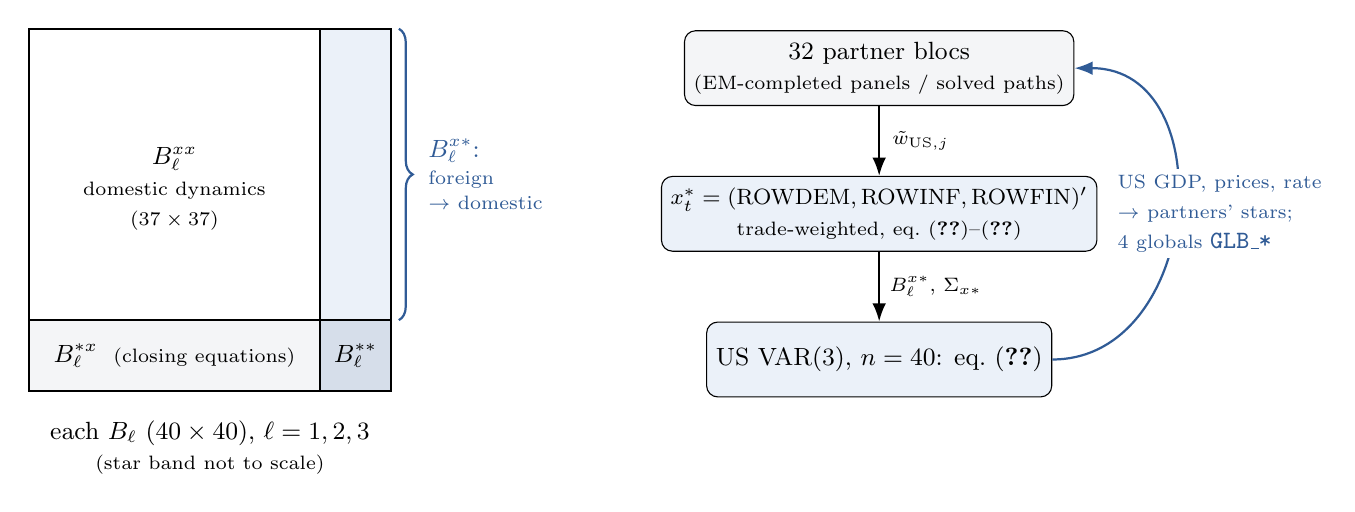
\begin{tikzpicture}[font=\small]
  % ---- left: block partition of B_ell (star band widened for legibility) ----
  \begin{scope}[shift={(0,0)}]
    \fill[blksoft]    (3.7,0.9) rectangle (4.6,4.6);  % B^{x*}
    \fill[blkgray]    (0,0)     rectangle (3.7,0.9);  % B^{*x}
    \fill[blkblue!20] (3.7,0)   rectangle (4.6,0.9);  % B^{**}
    \draw[thick] (0,0) rectangle (4.6,4.6);
    \draw[thick] (3.7,0) -- (3.7,4.6);
    \draw[thick] (0,0.9) -- (4.6,0.9);
    \node at (1.85,2.95) {$B^{xx}_\ell$};
    \node[align=center] at (1.85,2.35) {\scriptsize domestic dynamics\\ \scriptsize ($37\times37$)};
    \draw[decorate, decoration={brace, amplitude=5pt}, thick, blkblue]
      (4.7,4.6) -- (4.7,0.9);
    \node[align=left, text=blkblue, anchor=west] at (4.95,2.75)
      {$B^{x*}_\ell$:\\[-1pt] \scriptsize foreign\\[-2pt] \scriptsize $\to$ domestic};
    \node at (1.85,0.45) {$B^{*x}_\ell$\; {\scriptsize (closing equations)}};
    \node at (4.15,0.45) {$B^{**}_\ell$};
    \node[anchor=north, align=center] at (2.3,-0.25)
      {each $B_\ell$ ($40\times40$), $\ell=1,2,3$\\ \scriptsize (star band not to scale)};
  \end{scope}
  % ---- right: the linkage loop (feedback routed on the east side) ----
  \begin{scope}[shift={(8.4,0.0)}]
    \node[draw, rounded corners, fill=blkgray, align=center, minimum width=3.6cm, minimum height=0.95cm]
      (partners) at (2.4,4.1) {32 partner blocs\\ \scriptsize (EM-completed panels / solved paths)};
    \node[draw, rounded corners, fill=blksoft, align=center, minimum width=3.6cm, minimum height=0.95cm]
      (stars) at (2.4,2.25) {{\footnotesize $x^{*}_t=(\mathrm{ROWDEM},\mathrm{ROWINF},\mathrm{ROWFIN})'$}\\ \scriptsize trade-weighted, eq.~\eqref{eq:rowdem}--\eqref{eq:rowfin}};
    \node[draw, rounded corners, fill=blksoft, align=center, minimum width=3.6cm, minimum height=0.95cm]
      (usvar) at (2.4,0.4) {US VAR(3), $n=40$: eq.~\eqref{eq:blocks}};
    \draw[-{Latex}, thick] (partners) -- node[right, xshift=1pt] {\scriptsize $\tilde w_{\mathrm{US},j}$} (stars);
    \draw[-{Latex}, thick] (stars) -- node[right] {\scriptsize $B^{x*}_\ell$, $\Sigma_{x*}$} (usvar);
    \draw[-{Latex}, thick, blkblue] (usvar.east) .. controls +(1.9,0) and +(1.9,0) .. (partners.east);
    \node[fill=white, inner sep=2pt, align=left, text=blkblue, anchor=west] at (5.35,2.25)
      {\scriptsize US GDP, prices, rate\\ \scriptsize $\to$ partners' stars;\\ \scriptsize 4 globals \code{GLB\_*}};
  \end{scope}
\end{tikzpicture}}
\caption{\emph{Left:} where the foreign variables enter --- the shaded column block $B^{x*}_\ell$
gives each of the 37 domestic equations its nine foreign regressors; the bottom rows are the
stars' own (closing) equations. \emph{Right:} the two-way linkage. The US is both a receiver
(its stars aggregate its partners) and the source of the four global commons; the feedback loop is
closed at estimation time by the EM star iteration and at solve time by the fixed point of
Section~\ref{sec:solve}.}
\label{fig:partition}
\end{figure}

\subsection{Estimated objects and state-space form}\label{sec:ss}

Estimation is by the regression layout $y_t' = z_t'\beta + u_t'$ with
$z_t = (1, y_{t-1}', y_{t-2}', y_{t-3}')' \in \mathbb{R}^{121}$, so
$\beta = (c, B_1, B_2, B_3)' \in \mathbb{R}^{121\times40}$: the first row is the intercept, and
rows $2,\dots,121$ stack $B_1', B_2', B_3'$.\footnote{\code{bvarGLPmf.m:171--183};
the shipped posterior means are $\hat\beta$ (\code{betahat}, $121\times40$) and $\hat\Sigma$
(\code{sigmahat}, $40\times40$) in \code{companion\_mean.json}, together with all 500 retained
posterior draws in \code{companion\_draws.json(.gz)} (shapes $[121,40,500]$) from which the
tool's predictive bands are computed.} This layout (\code{seasonalRows}${}=0$) is exact for the
US and every seasonally-adjusted bloc; a minority of coupled blocs whose source series are not
seasonally adjusted instead carry three quarterly seasonal-dummy coefficients \emph{between} the
intercept and the lag blocks, so their $\hat\beta$ is
$[\,c;\ \gamma_{Q2};\ \gamma_{Q3};\ \gamma_{Q4};\ B_1;\dots;B_p\,]$ with \code{seasonalRows}${}=3$
--- which is why those blocs' \code{companion\_mean.json} ships extra rows --- and a few
coupon-lumpy fiscal blocs additionally have their interest payments evenly distributed within each
calendar year before estimation, so their \code{EFFI} is an accrual borrowing cost rather than a
coupon sawtooth. Neither device touches the US, whose panel is seasonally adjusted and whose
interest is not coupon-lumpy.\footnote{Seasonal-dummy layout and the \code{seasonalRows} tag:
\code{export\_bvar\_gvar24\_loop.m:331--355} ($\text{nsr}=\text{rows}(\hat\beta)-(1+np)$, asserted
$\in\{0,3\}$; \code{seasonalRows}, \code{qoyNext} exported to \code{spec.json} and
\code{companion\_mean.json}) and \code{app/src/lib/compute/kalman.ts:20--27, 62--71}. Even coupon
distribution: \code{EVEN\_INTEREST=\{CL,CO,CR,ID,IL,MX,TR,ZA\}} and \code{even\_distribute\_years}
in \code{pipeline/build\_fiscal22\_columns.py:58--61, 181}. Both are described in the seasonality
section of the companion user manual.} For forecasting and conditioning the tool puts \eqref{eq:var} in
companion (state-space) form,
\begin{equation}\label{eq:companion}
  \alpha_t = \mathbf{T}\,\alpha_{t-1} + c_\alpha + \eta_t, \qquad
  y^{\mathrm{obs}}_t = Z\,\alpha_t + \varepsilon_t,
\end{equation}
where $\alpha_t = (y_t', y_{t-1}', y_{t-2}')' \in \mathbb{R}^{120}$,
\[
  \mathbf{T} =
  \begin{pmatrix}
    B_1 & B_2 & B_3 \\
    I_{40} & 0 & 0 \\
    0 & I_{40} & 0
  \end{pmatrix},
  \qquad
  c_\alpha = \begin{pmatrix} c \\ 0 \\ 0 \end{pmatrix},
  \qquad
  Z = \begin{pmatrix} I_{40} & 0 & 0 \end{pmatrix},
\]
$\eta_t \sim \mathcal{N}(0, Q)$ with $\Sigma$ in the top-left $40\times40$ block of $Q$, and
$\varepsilon_t \sim \mathcal{N}(0, 10^{-12} I)$ --- the near-degenerate measurement noise that
implements \emph{hard} conditioning: any observed or pinned cell is matched essentially exactly,
and missing cells are simply dropped from the observation vector at that
date.\footnote{\code{app/src/lib/compute/kalman.ts:43--83} (state space, $R=10^{-12}$),
\code{kalman.ts:129--141} (missing cells dropped; a finite user-supplied variance overrides the
hard pin for \emph{soft} conditioning).}

\section{The foreign variables}\label{sec:stars}

\subsection{Trade weights}

The linkage weights are bilateral goods-trade shares (exports FOB plus imports CIF, IMF
International Merchandise Trade Statistics, 2021--2023 average), row-normalized over the other 32
coupled blocs with a zero diagonal.\footnote{\code{app/public/data/bvar/gvar/weights\_full.json}
(the estimator's input) and \code{weights\_24bloc.json} (the app runtime's input) --- numerically
identical, 33 blocs including the US row; builder \code{pipeline/build\_us\_weights\_row.py}
(partners below 0.05\% dropped, then renormalized).} The US row has 31 non-zero partners;
Table~\ref{tab:weights} shows the ten largest.

\begin{table}[h]
\centering
\caption{The US trade-weight row $w_{\mathrm{US},j}$ (top 10 of 31 partners; shipped values).}
\label{tab:weights}
\small
\begin{tabular}{lc@{\qquad}lc}
\toprule
Partner & $w_{\mathrm{US},j}$ & Partner & $w_{\mathrm{US},j}$ \\
\midrule
Euro area (EA) & 0.176351 & Korea (KR)          & 0.039860 \\
Mexico (MX)    & 0.168428 & United Kingdom (UK) & 0.029843 \\
Canada (CA)    & 0.168175 & Taiwan POC (TW)     & 0.028405 \\
China (CN)     & 0.144603 & India (IN)          & 0.027841 \\
Japan (JP)     & 0.049779 & Switzerland (CH)    & 0.019897 \\
\bottomrule
\end{tabular}
\end{table}

The weights are static (one row per bloc), but the weights actually applied are renormalized
\emph{per component and per quarter} over the partners available and eligible at that date:
\begin{equation}\label{eq:wtilde}
  \tilde w^{\,k}_{\mathrm{US},j,t}
  \;=\;
  \frac{w_{\mathrm{US},j}\;\mathbf{1}\{j \text{ eligible for component } k \text{ at } t\}}
       {\sum_{j'} w_{\mathrm{US},j'}\;\mathbf{1}\{j' \text{ eligible for } k \text{ at } t\}},
  \qquad k \in \{\mathrm{DEM}, \mathrm{INF}, \mathrm{FIN}\},
\end{equation}
so that missing partners' weight is reabsorbed by the rest. Eligibility differs by component:
a partner with no rate series at all (Switzerland, Norway, Brazil, Saudi Arabia) drops out of
$\mathrm{FIN}$ only, and Argentina --- whose 2023--24 hyperinflation would otherwise dominate the
price and rate moments --- is excluded from $\mathrm{INF}$ and $\mathrm{FIN}$ but kept in
$\mathrm{DEM}$.\footnote{Estimator:
\code{export\_bvar\_gvar24\_loop.m:189--217} (\code{buildstars}; the \code{xinf} exclusion at line
203). Runtime: \code{app/src/lib/compute/gvarSolve.ts:99--100, 244--273}
(\code{EXCLUDE\_INF\_FIN=\{AR\}}, \code{gvarPartnerWeights}). The estimator applies
\eqref{eq:wtilde} with per-quarter availability; the runtime applies the same per-component
renormalization with a static eligibility set --- per-quarter availability only matters for the
historical star construction.}

\subsection{Construction of the stars}

For each partner $j$ let $\ell^{g}_{j,t}$ and $\ell^{\pi}_{j,t}$ be the $100\ln$ levels of $j$'s
real GDP and consumer-price (or deflator) series, and $r_{j,t}$ its short rate in percent --- the
bloc's policy rate where one exists, else its 10-year government-bond yield (the fallback used
for the Czech Republic, Hungary, and Poland) --- all read from $j$'s \emph{EM-completed} panel
(the posterior-mean Durbin--Koopman completion of Section~\ref{sec:estimation}, not the raw
data). The three US stars are
\begin{align}
  \mathrm{ROWDEM}_t &= 4 \sum_{j \neq \mathrm{US}} \tilde w^{\,\mathrm{DEM}}_{\mathrm{US},j,t}
      \left( \ell^{g}_{j,t} - \ell^{g}_{j,t-1} \right),
      \label{eq:rowdem}\\
  \mathrm{ROWINF}_t &= 4 \sum_{j \neq \mathrm{US}} \tilde w^{\,\mathrm{INF}}_{\mathrm{US},j,t}
      \left( \ell^{\pi}_{j,t} - \ell^{\pi}_{j,t-1} \right),
      \label{eq:rowinf}\\
  \mathrm{ROWFIN}_t &= \phantom{4} \sum_{j \neq \mathrm{US}} \tilde w^{\,\mathrm{FIN}}_{\mathrm{US},j,t}\; r_{j,t}.
      \label{eq:rowfin}
\end{align}
$\mathrm{ROWDEM}$ and $\mathrm{ROWINF}$ are trade-weighted quarter-on-quarter \emph{annualized}
growth rates in percent --- the factor is $4$ on the $100\ln$ scale, i.e.\
$400\,\Delta\ln$, matching the tool's display convention --- while $\mathrm{ROWFIN}$ is a
\emph{level} average of partner rates (no differencing, no
annualization).\footnote{\code{export\_bvar\_gvar24\_loop.m:204--212}: \code{gd(t)=4*ad/wd},
\code{gi(t)=4*ai/wi}, \code{fr(t)=af/wf}. Leading missing values (quarters before a partner
set exists) are back-filled with the first valid value so no bloc carries a NaN prefix
(lines 213--217).} Partner GDP enters \eqref{eq:rowdem} as a chain-linked volume level, with one
legacy exception: the estimator's China branch deflates in $100\ln$ space
($\ell^{g}_{\mathrm{CN}} - \ell^{\pi}_{\mathrm{CN}}$), a convention retained from the vintage in
which China's panel carried nominal GDP.\footnote{\code{export\_bvar\_gvar24\_loop.m:184--185}
(\code{panelfrom}). The current China raw panel ships a chain-linked volume index, so this branch
is a reconciliation item for the next full re-estimation; the app runtime reads the (real) level
directly.}

Two conventions matter for estimation. First, over the COVID window the two macro stars
$\mathrm{ROWDEM}$ and $\mathrm{ROWINF}$ are set to missing along with the domestic macro block,
while $\mathrm{ROWFIN}$ stays observed --- partners' policy rates were genuinely observed through
2020 (Section~\ref{sec:estimation}). Second, the star \emph{history} is model-generated data: it
is rebuilt at every outer sweep from the partners' current completed panels, which is what makes
the estimated system a fixed point rather than a two-step plug-in.

\subsection{The global commons}\label{sec:globals}

Four of the 37 domestic columns are US-originated variables that every other bloc carries as
common exogenous drivers: the 10-year Treasury yield (\code{GLB\_USLR}), Moody's Baa yield
(\code{GLB\_USBAA}), a US equity price index (\code{GLB\_USEQ}), and the WTI oil price
(\code{GLB\_OIL}). In the US bloc they are ordinary endogenous columns of $x_t$; in every partner
bloc they appear as the same four series and are pinned, at solve time, to the US solution
(Section~\ref{sec:solve}). The US is thus the \emph{source} of the global commons and never a
receiver.\footnote{Spec blocks \code{"global"} at columns 23, 25, 27, 36 of
\code{app/public/data/bvar/US/spec.json}; the broadcast is \code{applyGlobalPins},
\code{gvarSolve.ts:479--497}, and is skipped for the US itself (lines 523--526).}

\section{The prior}\label{sec:prior}

The prior is the conjugate hierarchical Minnesota--normal--inverse-Wishart of
\citet{Giannone2015} (GLP), with the sum-of-coefficients extension of
\citet{DoanLittermanSims1984}:
\begin{equation}\label{eq:niw}
  \operatorname{vec}(\beta) \,\big|\, \Sigma \;\sim\;
  \mathcal{N}\!\big(\operatorname{vec}(b),\; \Sigma \otimes \Omega\big),
  \qquad
  \Sigma \;\sim\; \mathcal{IW}\!\big(\Psi,\, d\big), \qquad d = n+2 = 42 .
\end{equation}

\paragraph{Prior mean.} $b$ is zero except on the first own lag:
\begin{equation}\label{eq:priormean}
  b^{(1)}_{jj} = \delta_j, \qquad
  \delta_j =
  \begin{cases}
    0 & j \in \{\code{FREV\_GDP}, \code{FPEXP\_GDP}, \code{SFA}\} \quad (\text{white-noise prior}),\\
    1 & \text{otherwise} \quad (\text{random-walk prior}),
  \end{cases}
\end{equation}
i.e.\ the three fiscal GDP-ratios are shrunk toward stationarity around their means while all
other columns --- including the three stars --- carry the standard random-walk mean.\footnote{The
switch is the \code{pos} vector zeroing the own-lag diagonal, \code{bvarGLPmf.m:204--207}; the
tags come from the per-variable \code{prior} field of the panel spec
(\code{export\_bvar\_gvar24\_loop.m:55--60}). The effective interest rate \code{EFFI} stays RW.}

\paragraph{Prior variance.} $\Omega$ is diagonal. The intercept is diffuse,
$\Omega_{11} = V_c \approx 10^{6}$,\footnote{$V_c = 10^{7}$ in the marginal-likelihood evaluation
(\code{bvarGLPmf.m:33}) and $10^{6}$ in the posterior-draw function (\code{Support/BVAR.m:3});
both are diffuse and the discrepancy is numerically immaterial, but this note reports what the
code does.} and the coefficient of variable $j$ at lag $\ell$ has, in every equation,
\begin{equation}\label{eq:minnesota}
  \Omega_{(\ell,j)} \;=\; (d-n-1)\, \frac{\lambda^2}{\ell^{2}\,\psi_j}
  \;=\; \frac{\lambda^{2}}{\ell^{2}\,\psi_j},
\end{equation}
since $d-n-1 = 1$: overall tightness $\lambda$, harmonic lag decay with exponent 2, and scaling by
$\psi_j$, the residual variance of a univariate AR(1) fitted to column $j$. The inverse-Wishart
scale is $\Psi = (d-n-1)\operatorname{diag}(\psi) = \operatorname{diag}(\psi)$, so
$\mathbb{E}[\Sigma] = \operatorname{diag}(\psi)$. The $\psi_j$ are \emph{fixed} at their AR(1)
estimates (they are not sampled), and no dummy-initial-observation prior is
used.\footnote{\code{MNpsi=0}, \code{sur=0} in the estimator call,
\code{export\_bvar\_gvar24\_loop.m:107,141}; the $\Omega$ and $\Psi$ formulas are
\code{Support/BVAR.m:29--57} and \code{logMLMFVAR.m:38--63}.}

\paragraph{Sum-of-coefficients dummies.} The ``no-cointegration'' (\code{noc}) prior is
implemented by one artificial observation per variable, with weight $1/\mu$,
\[
  Y_d = \operatorname{diag}(\bar y_0)/\mu, \qquad
  X_d = \big[\,0,\; \operatorname{diag}(\bar y_0)/\mu,\;
              \operatorname{diag}(\bar y_0)/\mu,\; \operatorname{diag}(\bar y_0)/\mu\,\big],
\]
where $\bar y_0$ is the mean of the first $p$ rows of the \emph{regression} sample (observations
$p{+}1, \dots, 2p$ of the panel; 1999Q2--1999Q4). For the three white-noise variables the $Y_d$
rows are zeroed while $X_d$ keeps $\operatorname{diag}(\bar y_0)/\mu$, so their dummy observation
pulls each equation's \emph{total} lag loading on them toward zero rather than one --- consistent
with the $\delta_j = 0$ prior mean, not an exemption from the
dummies.\footnote{\code{Support/BVAR.m:20--22, 62--66}; \code{ydnoc(pos,pos)=0} zeroes only the
left-hand side.}

\paragraph{Hyperpriors.} The two shrinkage hyperparameters are themselves estimated:
\begin{equation}\label{eq:hyper}
  \lambda \sim \Gamma(\text{mode } 0.2,\ \text{sd } 0.4), \qquad
  \mu \sim \Gamma(\text{mode } 1,\ \text{sd } 1),
\end{equation}
with support truncated to $[10^{-4}, 5]$, and are sampled by a random-walk Metropolis step on the
marginal likelihood of the \emph{completed} data (Section~\ref{sec:estimation}). The proposal
covariance is the inverse Hessian of the \code{csminwel} hyperparameter-posterior maximization
with its eigenvalues capped, and the chain starts from a draw around that mode reflected into the
support box.\footnote{\code{cgl\_bvarV5.m:31--37, 66--84, 108--117, 151--166}.}

\section{Estimation with incomplete data}\label{sec:estimation}

\subsection{The missing-data pattern}

Interior holes --- the pandemic quarters, and interior gaps such as a handful of missing
\code{SFA} cells --- are treated as missing data, never as dummies. Two boundary conventions
apply: leading-edge gaps (including the first row of the constructed stars) are back-filled with
the first valid value, and the likelihood sample is cut at the last fully-observed row of the
completed panel --- a no-op for the US, whose panel is complete over 1998Q3--2025Q4.
The COVID window is fixed at 2020Q2--2020Q4 and
masks \emph{macro} cells only: all domestic columns with \code{isFinancial}${}=0$ plus the two
macro stars $\mathrm{ROWDEM}, \mathrm{ROWINF}$ are set to missing there, while financial columns
(rates, yields, equity, house prices, credit) and $\mathrm{ROWFIN}$ remain
observed.\footnote{\code{export\_bvar\_gvar24\_loop.m:83--90, 130--137}. This differs from the
outlier-variance treatment of \citet{LenzaPrimiceri2022}: here the pandemic macro observations
are simply \emph{not data}, and their imputation is conditioned on the financial columns that
are.} Because imputation is per cell, the observed financials discipline the imputed macros
within the same quarter.

\subsection{The Gibbs sampler}

Estimation is a data-augmentation sampler in the spirit of \citet{TannerWong1987}, run for
1{,}000 sweeps (500 burn-in). Each sweep $g$:
\begin{enumerate}[leftmargin=1.8em, itemsep=1pt]
  \item \emph{Completion draw.} Draw the missing cells with the Durbin--Koopman simulation
        smoother \citep{DurbinKoopman2002} on the companion form \eqref{eq:companion}: simulate an
        artificial path, smooth the difference, and add back, yielding a completed panel
        $\tilde y^{(g)}$. One implementation detail matters for exactness: the smoother's
        companion matrices are built \emph{once}, from the \code{csminwel} posterior-mode fit
        $(\hat\beta_{\mathrm{mode}}, \hat\Sigma_{\mathrm{mode}})$, and are not updated across
        sweeps --- only the artificial path's innovations use the current $\Sigma$ draw. The
        imputed cells are therefore draws from
        $p(y^{\mathrm{miss}} \mid y^{\mathrm{obs}}, \hat\beta_{\mathrm{mode}},
        \hat\Sigma_{\mathrm{mode}})$, a \emph{fixed-companion approximation} to full data
        augmentation rather than conditioning on the previous sweep's coefficient
        draw.\footnote{\code{cgl\_bvarV5.m:85--95} (companion built from \code{r.postmax} before
        the loop and never reassigned inside it) and \code{:127--145} (the DK draw). Steps 2--3
        condition on this completion exactly.}
  \item \emph{Hyperparameter step.} Update $(\lambda, \mu)$ by random-walk Metropolis on the
        marginal likelihood $p(\tilde y^{(g)} \mid \lambda, \mu)$ of the completed data under
        \eqref{eq:niw}--\eqref{eq:hyper}.
  \item \emph{Coefficient step.} Draw $(\beta, \Sigma)^{(g)}$ from the conjugate
        normal--inverse-Wishart posterior given $\tilde y^{(g)}$ and $(\lambda, \mu)^{(g)}$,
        including the sum-of-coefficients dummies.
\end{enumerate}
The shipped point model is the posterior mean over the 500 retained draws ---
$\hat\beta = \overline{\beta^{(g)}}$, $\hat\Sigma = \overline{\Sigma^{(g)}}$ --- and the 500
individual draws ship alongside it for the predictive bands.\footnote{\code{cgl\_bvarV5.m:127--205}
(the three steps), \code{export\_bvar\_gvar24\_loop.m:229--247} (export).}

\subsection{The outer star iteration}\label{sec:emloop}

The star columns \eqref{eq:rowdem}--\eqref{eq:rowfin} are inputs to the US estimation but outputs
of the partners' estimations --- so the whole system is iterated to a fixed point. Each outer
sweep $m$ (a \emph{Jacobi} sweep: all 33 blocs are re-estimated in parallel against the stars
built from the sweep-$(m-1)$ completions):
\[
  \text{completed panels}^{(m-1)}
  \;\xrightarrow{\ \eqref{eq:rowdem}-\eqref{eq:rowfin}\ }\;
  \text{stars}^{(m)}
  \;\xrightarrow{\ \text{Gibbs above}\ }\;
  \text{completed panels}^{(m)},
\]
with convergence declared when
\begin{equation}\label{eq:emtol}
  \max_{c,\,k,\,t} \big| \mathrm{star}^{(m)}_{c,k,t} - \mathrm{star}^{(m-1)}_{c,k,t} \big| \;<\; 0.03
\end{equation}
(annualized percentage points), the COVID rows of the two macro stars excluded from the metric
because their sweep-to-sweep churn is imputation Monte-Carlo noise; the cap is 12
sweeps.\footnote{\code{export\_bvar\_gvar24\_loop.m:122--157}. The US enters this loop as an
ordinary bloc --- \code{US\_ENDOGENOUS=1} --- after one closed no-stars estimation that seeds the
first sweep; that warm-start fit is discarded, not shipped (lines 95--117).} At the fixed point
every bloc's stars are consistent with every other bloc's completed history --- the estimation-time
counterpart of the solve-time fixed point below.

\section{The estimated foreign block}\label{sec:loadings}

Table~\ref{tab:loadings} reports the posterior-mean loadings of four representative US equations
on the three stars --- selected rows of $B^{x*}_\ell$ in \eqref{eq:blocks} --- together with the
innovation correlations from $\hat\Sigma$. Units matter when reading the numbers: log variables
(GDP, exports) are $100\ln$ \emph{levels}, so a coefficient of $0.042$ on lagged
$\mathrm{ROWDEM}$ means that one percentage point of additional annualized foreign growth for one
quarter raises the US GDP level by $0.042$ percent (about $0.17$ percentage points of annualized
growth in that quarter); rate equations (federal funds, 10-year) are in percent per annum.

\begin{table}[h]
\centering
\caption{Posterior-mean star loadings of selected US equations, and innovation correlations.
Recomputed from the shipped \code{companion\_mean.json}.}
\label{tab:loadings}
\small
\begin{tabular}{llrrrr}
\toprule
Equation & Star regressor & Lag 1 & Lag 2 & Lag 3 & $\sum_\ell$ \\
\midrule
Real GDP (\code{GDPH})      & $\mathrm{ROWDEM}$ & $+0.042$ & $-0.006$ & $-0.012$ & $+0.024$ \\
                            & $\mathrm{ROWINF}$ & $+0.053$ & $+0.004$ & $-0.001$ & $+0.056$ \\
                            & $\mathrm{ROWFIN}$ & $-0.462$ & $+0.308$ & $-0.016$ & $-0.170$ \\
\addlinespace
CPI (\code{UI})             & $\mathrm{ROWDEM}$ & $+0.026$ & $+0.004$ & $-0.024$ & $+0.007$ \\
                            & $\mathrm{ROWINF}$ & $+0.072$ & $+0.010$ & $+0.012$ & $+0.095$ \\
                            & $\mathrm{ROWFIN}$ & $+0.110$ & $-0.064$ & $-0.083$ & $-0.036$ \\
\addlinespace
Federal funds (\code{POLRATE}) & $\mathrm{ROWDEM}$ & $+0.014$ & $-0.011$ & $-0.003$ & $-0.000$ \\
                            & $\mathrm{ROWINF}$ & $+0.021$ & $-0.026$ & $+0.012$ & $+0.007$ \\
                            & $\mathrm{ROWFIN}$ & $-0.086$ & $+0.009$ & $+0.045$ & $-0.032$ \\
\addlinespace
Real exports (\code{XH})    & $\mathrm{ROWDEM}$ & $+0.072$ & $+0.098$ & $+0.044$ & $+0.214$ \\
                            & $\mathrm{ROWINF}$ & $-0.135$ & $-0.048$ & $-0.075$ & $-0.258$ \\
                            & $\mathrm{ROWFIN}$ & $-0.400$ & $-0.010$ & $-0.318$ & $-0.729$ \\
\midrule
\multicolumn{6}{l}{\emph{Innovation correlations (from $\hat\Sigma$):}\quad
  $\operatorname{corr}(u_{\mathrm{GDPH}}, u_{\mathrm{ROWDEM}}) = 0.49$;\quad
  $\operatorname{corr}(u_{\mathrm{UI}}, u_{\mathrm{ROWINF}}) = 0.54$;} \\
\multicolumn{6}{l}{\quad
  $\operatorname{corr}(u_{\mathrm{JGDP}}, u_{\mathrm{ROWINF}}) = 0.43$;\quad
  $\operatorname{corr}(u_{\mathrm{POLRATE}}, u_{\mathrm{ROWFIN}}) = 0.27$;\quad
  $\operatorname{corr}(u_{\mathrm{XH}}, u_{\mathrm{ROWDEM}}) = 0.18$.} \\
\midrule
\multicolumn{6}{l}{\emph{Star own-lag persistence (rows of $B^{**}_\ell$):}\quad
  $\mathrm{ROWDEM}$: $0.64, -0.11, -0.15$ ($\sum = 0.38$);} \\
\multicolumn{6}{l}{\quad
  $\mathrm{ROWINF}$: $0.05, -0.19, +0.01$ ($\sum = -0.14$);\quad
  $\mathrm{ROWFIN}$: $0.66, +0.01, -0.05$ ($\sum = 0.62$).} \\
\bottomrule
\end{tabular}
\end{table}

The pattern is economically coherent: exports load positively and persistently on foreign demand
($\sum_\ell = 0.21$) and negatively on foreign rates; the same-quarter co-movement of US GDP with
foreign demand ($0.49$) and of US consumer prices with foreign inflation ($0.54$) runs through
$\Sigma_{x*}$, which is precisely the covariance the conditional-forecast smoother exploits when
a star path is pinned. Among the star equations themselves, the foreign rate is the persistent
one (own-lag sum $0.62$), while trade-weighted foreign inflation is close to white noise in its
annualized quarterly form.

\section{The linkage at solve time}\label{sec:solve}

\subsection{Scenarios are conditional forecasts}

A forecast in the tool is the smoothed mean of \eqref{eq:companion}; a scenario adds \emph{pins}
--- future observations $y^{\mathrm{obs}}_{i,T+h}$ placed on any cell --- and the Durbin--Koopman
smoother moves every free variable to its conditional expectation given all pins, exactly in the
tradition of conditional VAR forecasting \citep{WaggonerZha1999,BanburaGiannoneLenza2015}. Hard
pins carry the $10^{-12}$ measurement variance of Section~\ref{sec:ss}; soft pins (e.g.\ external
forecasts with a trust dial) replace it with a finite variance.

\subsection{Pinning the stars to the partners}

In a coupled (``global'') solve the US star paths are not left to the closing equations: for every
projection step $h = 1, \dots, 20$ they are hard-pinned to
\begin{equation}\label{eq:starpin}
  x^{*,\mathrm{pin}}_{\mathrm{US},k,T+h}
  \;=\;
  \bar x^{*}_{\mathrm{US},k,T+h} \;+\; \Delta^{*}_{\mathrm{US},k,T+h},
\end{equation}
the bloc's own \emph{unconditional} star forecast $\bar x^{*}$ plus a trade-weighted sum of the
partners' \emph{deviations} from their own unconditional baselines:
\begin{align}
  \Delta^{*}_{\mathrm{US},\mathrm{DEM},T+h}
    &= \sum_{j} \tilde w^{\,\mathrm{DEM}}_{\mathrm{US},j}\; 4\Big[
        \big(\ell^{g,\mathrm{scen}}_{j,T+h} - \ell^{g,\mathrm{scen}}_{j,T+h-1}\big)
      - \big(\bar\ell^{g}_{j,T+h} - \bar\ell^{g}_{j,T+h-1}\big) \Big],
      \label{eq:demdelta}\\
  \Delta^{*}_{\mathrm{US},\mathrm{FIN},T+h}
    &= \sum_{j} \tilde w^{\,\mathrm{FIN}}_{\mathrm{US},j}\;
        \big( r^{\mathrm{scen}}_{j,T+h} - \bar r_{j,T+h} \big),
      \label{eq:findelta}
\end{align}
and $\Delta^{*}_{\mathrm{INF}}$ as \eqref{eq:demdelta} on the price levels. At $h=1$ both
back-differences are anchored at the shared panel-origin row (2026Q1 --- observed for the US, a
cross-bloc nowcast for the other blocs), so the bracketed term in \eqref{eq:demdelta} collapses to
the level gap $\ell^{g,\mathrm{scen}}_{j,T+1} - \bar\ell^{g}_{j,T+1}$. Deviations --- not levels --- are what travel
between blocs: each bloc keeps its own estimated baseline, and only news relative to baseline
propagates.\footnote{\code{gvarSolve.ts:424--453} (\code{rowPinDelta}) and \code{499--528}
(\code{buildCondPaths}); the readout column per component mirrors the estimator's series choice
(GDP, CPI/deflator, policy rate), \code{gvarSolve.ts:106--124, 239}.} Symmetrically, every partner
bloc $c$ has its own $\mathrm{ROW*}_{c}$ stars pinned the same way --- with the US as one of its
partners --- and its four global commons pinned to the US deviation:
\begin{equation}\label{eq:globpin}
  z^{\mathrm{pin}}_{c,g,T+h} = \bar z_{c,g,T+h}
    + \big( z^{\mathrm{scen}}_{\mathrm{US},g,T+h} - \bar z_{\mathrm{US},g,T+h} \big),
  \qquad g \in \{\code{GLB\_USLR}, \code{GLB\_USBAA}, \code{GLB\_USEQ}, \code{GLB\_OIL}\}.
\end{equation}

\subsection{The linear fixed point}

Because $(\hat\beta, \hat\Sigma)$ are fixed at solve time, the smoothed conditional forecast is
\emph{affine} in the pinned values --- so the mutual consistency of all 33 blocs is a linear
problem. Stack the unknown star deviations of every coupled bloc and the US global deviations
into
\[
  x \;=\; \Big( \big\{\Delta^{*}_{c,k,T+h}\big\}_{c=1..33,\;k=1..3,\;h=1..20},\;\;
                \big\{\Delta^{\mathrm{GLB}}_{g,T+h}\big\}_{g=1..4,\;h=1..20} \Big)
  \;\in\; \mathbb{R}^{2060},
\]
($33\times3\times20 + 4\times20 = 2060$). Propagating any candidate $x$ through every bloc's
smoother and re-reading the partners' responses is an affine map, giving the fixed-point equation
\begin{equation}\label{eq:fp}
  x \;=\; M x + d,
\end{equation}
where $d$ collects the exogenous forcing (the user's own pins in each bloc, mapped to the
deviations they cause), and $M$ --- built column-by-column from unit-pin smoother kernels --- has
spectral radius
\begin{equation}\label{eq:rho}
  \rho(M) \;=\; 0.9466 \;<\; 1,
\end{equation}
so the solution $x = (I - M)^{-1} d$ exists, is unique, and equals the limit of iterating the
blocs to mutual consistency.\footnote{Computed by direct eigendecomposition of the shipped $M$;
the dominant eigenvalues are the complex pair $0.9446 \pm 0.0305i$. Before 2026-07-17 the
artifact's \code{rhoSpectral} field read $0.935044$, produced by a power iteration on $M^2$ that
does not converge on a complex dominant pair; the estimator and the shipped field (now
$0.945494$) were corrected on that date. Everything that matters analytically is that
$\rho(M) < 1$.} The $2060\times2060$ inverse is
precomputed once and shipped with the app, keyed to the \emph{empty} pin structure: it serves the
unconditioned global solve --- and drift-only scenarios, which move only $d$ --- as a single
matrix--vector product. Any hard-pinned scenario changes the pin structure, re-keys $M$, and is
solved by the inverse-free Neumann iteration $x \leftarrow d + Mx$ on a freshly assembled
(kernel-cached) $M$; soft pins force a Gauss--Seidel sweep over the blocs, because the closed-form
kernels assume hard pins.\footnote{\code{gvarSolve.ts:1112--1494} (\code{buildLinearSystemEndo},
\code{solveGVARClosedFormEndo}); artifact
\code{app/public/data/bvar/gvar/coupling\_default.json.gz} (\code{dim}: 2060, \code{pinStructure}:
empty, $M$ and $(I-M)^{-1}$ at 6 significant digits); producer
\code{app/scripts/precompute\_gvar\_coupling.mjs}; routing \code{runGvarSolve.ts:229--253}.
Affinity of the smoother in the pin values for a fixed pin mask: \code{kalman.ts:479--504}.}
After solving \eqref{eq:fp}, each bloc runs one final conditional forecast with its stars and
globals pinned to \eqref{eq:starpin}--\eqref{eq:globpin}, so every displayed variable is
consistent with the fixed point. The blocs are aligned by \emph{projection step}, not calendar
date: the blocs share the uniform 2026Q1 origin, so step $h$ is the same quarter everywhere ---
with one documented exception, Israel, whose rows sit on its own calendar (origin 2025Q1) and
which is coupled by row with a four-quarter offset pending its data
re-pull.\footnote{\code{app/src/lib/dates.ts:57--69}.}

\subsection{What endogeneity buys}

Since the US participates in $x$ with its own sixty star-deviation entries, a shock anywhere in
the system feeds back to the United States: a scenario that depresses euro-area demand lowers
$\mathrm{ROWDEM}_{\mathrm{US}}$ through \eqref{eq:demdelta}, moves US GDP through
$B^{x*}_\ell$ and $\Sigma_{x*}$, and the US response then re-enters every partner's stars and the
four global commons --- the Rest-of-World$\to$US channel that a frozen weakly-exogenous anchor
cannot represent. With the legacy frozen-anchor configuration the same architecture degrades
gracefully: the US drops out of $x$, and the system solves with one-way US$\to$world
transmission only.

\section{Relation to the classical GVAR}\label{sec:pesaran}

Table~\ref{tab:pesaran} summarizes the mapping to \citet{PesaranSchuermannWeiner2004},
\citet{DeesDiMauroPesaranSmith2007}, and the survey treatment of \citet{ChudikPesaran2016}.

\begin{table}[h]
\centering
\caption{The US bloc versus the classical GVAR country model.}
\label{tab:pesaran}
\small
\begin{tabular}{p{2.6cm}p{5.6cm}p{5.9cm}}
\toprule
 & Classical GVAR (VARX\textsuperscript{*}) & MFFM US bloc \\
\midrule
Foreign variables &
$x^*_t$ on the right-hand side with contemporaneous and lagged terms
($\Lambda_0 x^*_t + \Lambda_1 x^*_{t-1}$), assumed weakly exogenous (tested per bloc) &
$x^*_t$ endogenous columns with their own equations; linkage through lagged $B^{x*}_\ell$ and
the innovation covariance $\Sigma_{x*}$; no weak-exogeneity assumption for the US \\
\addlinespace
Estimation &
Equation-by-equation OLS / reduced-rank ML, each bloc on its own sample &
Hierarchical Bayes (GLP) with missing-data completion, iterated with the partners to the star
fixed point \eqref{eq:emtol} \\
\addlinespace
Missing data &
Common solve window; ragged edges truncated &
2020Q2--Q4 macro cells and interior gaps imputed by the DK smoother inside estimation;
ragged panel starts kept \\
\addlinespace
Dominant unit &
US model restricted; US weakly exogenous to the rest &
US fully endogenous, with its own stars and a trade-weight row; RoW$\to$US feedback \\
\addlinespace
Global solve &
Stack link matrices, invert $G_0$ once: $x_t = G_0^{-1}(a + \sum_\ell G_\ell x_{t-\ell} + u_t)$ &
Deviation fixed point $x = Mx + d$ in pin space, $\rho(M)=0.947$; pre-shipped $(I-M)^{-1}$;
scenario-time conditioning via the DK smoother \\
\bottomrule
\end{tabular}
\end{table}

\section{The model in numbers}

\begin{table}[h]
\centering
\caption{The shipped US bloc at a glance.}
\label{tab:numbers}
\small
\begin{tabular}{l p{9.6cm}}
\toprule
Endogenous variables $n$ & 40 \ (37 domestic + 3 stars) \\
Lags $p$ / horizon $H$ & 3 / 20 quarters \\
Estimation sample & 1998Q3--2025Q4 \ ($T = 110$); display origin 2026Q1 \\
Forecast window shown & 2026Q2--2031Q1 \\
COVID missing window & 2020Q2--2020Q4, macro cells only \\
Posterior draws & 1{,}000 Gibbs sweeps, 500 retained (shipped) \\
Prior & GLP Minnesota--NIW; $\lambda \sim \Gamma(0.2, 0.4)$, $\mu \sim \Gamma(1,1)$ (mode, sd) \\
White-noise columns & \code{FREV\_GDP}, \code{FPEXP\_GDP}, \code{SFA} \\
Trade weights & IMF IMTS 2021--23 average; 31 partners; EA 0.176, MX 0.168, CA 0.168, CN 0.145 \\
Global commons sourced & \code{GLB\_USLR}, \code{GLB\_USBAA}, \code{GLB\_USEQ}, \code{GLB\_OIL} \\
Coupled system & 33 blocs; state dim $2060$; $\rho(M) = 0.945494$ (eigendecomposition-exact;
see the footnote to eq.~\eqref{eq:rho}); $(I-M)^{-1}$ pre-shipped \\
Hard-pin measurement variance & $10^{-12}$ \\
\bottomrule
\end{tabular}
\end{table}

\clearpage
\appendix

\section{The 40-variable roster}\label{app:roster}

Order, mnemonics, spaces, and priors as shipped in \code{app/public/data/bvar/US/spec.json}.
Descriptions are from the estimation panel \code{DataRaw\_US\_glob.json}, and the source
mnemonics are from the shipped \code{coverage\_manifest.json}. \emph{Space}:
$100\ln$ = enters as $100\ln(\text{level})$, displayed as $4\Delta$ annualized growth (five index-type
series display as levels); level = enters untransformed (percent, percent of GDP, or index points).
\emph{Prior}: RW = random-walk own-lag mean 1; WN = white-noise own-lag mean 0, eq.~\eqref{eq:priormean}.

\begin{small}
\setlength{\tabcolsep}{4pt}
\begin{longtable}{r l p{5.9cm} c c c p{3.4cm}}
\caption{The US variable roster, in shipped order.}\label{tab:roster}\\
\toprule
\# & Mnemonic & Description & Space & Prior & Block & Source \\
\midrule
\endfirsthead
\toprule
\# & Mnemonic & Description & Space & Prior & Block & Source \\
\midrule
\endhead
\bottomrule
\endfoot
0 & \texttt{GDPH} & Real Gross Domestic Product & $100\ln$ & RW & macro & FRED GDPC1 \\
1 & \texttt{CH} & Real Personal Consumption Expenditures & $100\ln$ & RW & macro & FRED PCECC96 \\
2 & \texttt{FRH} & Real Private Residential Fixed Investment (nominal, deflated) & $100\ln$ & RW & macro & FRED PRFI / GDPDEF \\
3 & \texttt{FNH} & Real Private Nonresidential Fixed Investment (nominal, deflated) & $100\ln$ & RW & macro & FRED PNFI / GDPDEF \\
4 & \texttt{XH} & Real Exports of Goods \& Services & $100\ln$ & RW & macro & FRED EXPGSC1 \\
5 & \texttt{MH} & Real Imports of Goods \& Services & $100\ln$ & RW & macro & FRED IMPGSC1 \\
6 & \texttt{GH} & Real Government Consumption \& Gross Investment & $100\ln$ & RW & macro & FRED GCEC1 \\
7 & \texttt{JGDP} & GDP Chain Price Index & $100\ln$ & RW & macro & FRED GDPDEF \\
8 & \texttt{JC} & PCE Chain Price Index & $100\ln$ & RW & macro & FRED PCEPI \\
9 & \texttt{JCXFE} & PCE less Food \& Energy Price Index & $100\ln$ & RW & macro & FRED PCEPILFE \\
10 & \texttt{UI} & CPI-U: All Items & $100\ln$ & RW & macro & FRED CPIAUCSL \\
11 & \texttt{UIXFDG} & CPI-U: All Items Less Food \& Energy & $100\ln$ & RW & macro & FRED CPILFESL \\
12 & \texttt{LXBC} & Business Sector Compensation Per Hour (nominal) & $100\ln$ & RW & macro & FRED HCOMPBS \\
13 & \texttt{LANAGRA} & All Employees: Total Nonfarm & $100\ln$ & RW & macro & FRED PAYEMS \\
14 & \texttt{LR} & Civilian Unemployment Rate & level & RW & macro & FRED UNRATE \\
15 & \texttt{IP} & Industrial Production Index & $100\ln$ & RW & macro & FRED INDPRO \\
16 & \texttt{CUMFG} & Capacity Utilization: Manufacturing & level & RW & macro & FRED MCUMFN \\
17 & \texttt{HST} & Housing Starts & $100\ln$ & RW & macro & FRED HOUST \\
18 & \texttt{YPDH} & Real Disposable Personal Income & $100\ln$ & RW & macro & FRED DPIC96 \\
19 & \texttt{CSENT} & U.\ Michigan Consumer Sentiment & level & RW & macro & FRED UMCSENT \\
20 & \texttt{POLRATE} & Effective Federal Funds Rate & level & RW & fin. & FRED FEDFUNDS \\
21 & \texttt{FCM2} & 2-Year Treasury Yield (constant maturity) & level & RW & fin. & FRED DGS2 \\
22 & \texttt{FCM5} & 5-Year Treasury Yield (constant maturity) & level & RW & fin. & FRED DGS5 \\
23 & \texttt{GLB\_USLR} & 10-Year Treasury Yield (constant maturity) & level & RW & global & FRED DGS10 \\
24 & \texttt{FAAA} & Moody's Seasoned Aaa Corporate Yield & level & RW & fin. & FRED AAA \\
25 & \texttt{GLB\_USBAA} & Moody's Seasoned Baa Corporate Yield & level & RW & global & FRED BAA \\
26 & \texttt{FXTWM} & Trade-weighted US\$ index (advanced foreign economies) & $100\ln$ & RW & fin. & FRED DTWEXAFEGS (spliced onto DTWEXM) \\
27 & \texttt{GLB\_USEQ} & US equity price index & $100\ln$ & RW & global & FRED SPASTT01USM661N \\
28 & \texttt{GSNE} & IMF non-fuel commodity price index & $100\ln$ & RW & fin. & FRED PNFUELINDEXM \\
29 & \texttt{SP500VOL} & CBOE VIX & level & RW & fin. & FRED VIXCLS \\
30 & \texttt{HP} & Case--Shiller national house price index & $100\ln$ & RW & fin. & FRED CSUSHPISA \\
31 & \texttt{LEV} & Real nonfinancial business debt & $100\ln$ & RW & fin. & FRED BCNSDODNS / GDPDEF \\
32 & \texttt{FREV\_GDP} & Federal receipts (\% of GDP) & level & WN & fiscal & FRED FGRECPT / GDP \\
33 & \texttt{FPEXP\_GDP} & Federal primary expenditure (\% of GDP) & level & WN & fiscal & FRED FGEXPND, A091RC1Q027SBEA, GDP \\
34 & \texttt{EFFI} & Federal effective interest rate (\% p.a.) & level & RW & fiscal & FRED A091RC1Q027SBEA, GFDEGDQ188S \\
35 & \texttt{SFA} & Stock-flow adjustment (\% of GDP) & level & WN & fiscal & debt-identity residual \\
36 & \texttt{GLB\_OIL} & WTI crude oil price (quarterly average) & $100\ln$ & RW & global & FRED WTISPLC \\
37 & \texttt{ROWDEM\_US} & Foreign demand: trade-weighted partner real-GDP growth, eq.~\eqref{eq:rowdem} & level & RW & star & constructed \\
38 & \texttt{ROWINF\_US} & Foreign inflation: trade-weighted partner inflation, eq.~\eqref{eq:rowinf} & level & RW & star & constructed \\
39 & \texttt{ROWFIN\_US} & Foreign rate: trade-weighted partner policy rate, eq.~\eqref{eq:rowfin} & level & RW & star & constructed \\
\end{longtable}
\end{small}

\bibliographystyle{plainnat}
\bibliography{references}

\end{document}
